% TransferGap -- anonymized CoRL 2026 Scaling H2R workshop short paper.
% Build: tectonic main.tex (or latexmk -pdf main.tex).
% Numeric provenance: figures/number_sources.txt; review_recount.py.
\documentclass{article}
\usepackage{corl_2026}
\usepackage[T1]{fontenc}
\usepackage{graphicx}
\usepackage{booktabs}
\usepackage{amsmath,amssymb}
\usepackage{xcolor}
\usepackage{microtype}

\newcommand{\pp}{\,pp}
% AUTO-GENERATED by paper/make_figures.py from transfergap/results/ and paper/data/diagnosis_dev_snapshot.json -- do not edit.
\newcommand{\fiveDevFullK}{33}
\newcommand{\fiveDevFullN}{60}
\newcommand{\fiveDevFullPct}{55}
\newcommand{\fiveDevFullLo}{42}
\newcommand{\fiveDevFullHi}{67}
\newcommand{\fiveDevOPerceptionK}{41}
\newcommand{\fiveDevOPerceptionN}{60}
\newcommand{\fiveDevOPerceptionPct}{68}
\newcommand{\fiveDevOPerceptionLo}{56}
\newcommand{\fiveDevOPerceptionHi}{79}
\newcommand{\fiveDevORetargetingK}{30}
\newcommand{\fiveDevORetargetingN}{60}
\newcommand{\fiveDevORetargetingPct}{50}
\newcommand{\fiveDevORetargetingLo}{38}
\newcommand{\fiveDevORetargetingHi}{62}
\newcommand{\fiveDevOCalibrationK}{41}
\newcommand{\fiveDevOCalibrationN}{60}
\newcommand{\fiveDevOCalibrationPct}{68}
\newcommand{\fiveDevOCalibrationLo}{56}
\newcommand{\fiveDevOCalibrationHi}{79}
\newcommand{\fiveDevOTimingK}{39}
\newcommand{\fiveDevOTimingN}{60}
\newcommand{\fiveDevOTimingPct}{65}
\newcommand{\fiveDevOTimingLo}{52}
\newcommand{\fiveDevOTimingHi}{76}
\newcommand{\fiveDevOAllK}{60}
\newcommand{\fiveDevOAllN}{60}
\newcommand{\fiveDevOAllPct}{100}
\newcommand{\fiveDevOAllLo}{94}
\newcommand{\fiveDevOAllHi}{100}
\newcommand{\fiveBudPerception}{+13.3}
\newcommand{\fiveBudPerceptionLo}{+3.3}
\newcommand{\fiveBudPerceptionHi}{+23.3}
\newcommand{\fiveBudRetargeting}{$-$5.0}
\newcommand{\fiveBudRetargetingLo}{$-$15.0}
\newcommand{\fiveBudRetargetingHi}{+5.0}
\newcommand{\fiveBudCalibration}{+13.3}
\newcommand{\fiveBudCalibrationLo}{+1.7}
\newcommand{\fiveBudCalibrationHi}{+26.7}
\newcommand{\fiveBudTiming}{+10.0}
\newcommand{\fiveBudTimingLo}{+0.0}
\newcommand{\fiveBudTimingHi}{+20.0}
\newcommand{\fiveBudAll}{+45.0}
\newcommand{\fiveBudAllLo}{+33.3}
\newcommand{\fiveBudAllHi}{+58.3}
\newcommand{\fiveBudSum}{+31.7}
\newcommand{\fiveBudSumMinusAll}{$-$13.3}
\newcommand{\fiveBudIntAbs}{13.3}
\newcommand{\fiveHoFullK}{31}
\newcommand{\fiveHoFullN}{60}
\newcommand{\fiveHoFullPct}{52}
\newcommand{\fiveHoFullLo}{39}
\newcommand{\fiveHoFullHi}{64}
\newcommand{\fiveHoFullNoLift}{25}
\newcommand{\fiveHoFullNotPlaced}{29}
\newcommand{\fiveHoCorrK}{50}
\newcommand{\fiveHoCorrN}{60}
\newcommand{\fiveHoCorrPct}{83}
\newcommand{\fiveHoCorrLo}{72}
\newcommand{\fiveHoCorrHi}{91}
\newcommand{\fiveHoCorrNoLift}{8}
\newcommand{\fiveHoCorrNotPlaced}{10}
\newcommand{\fiveHoGap}{+31.7}
\newcommand{\fiveHoGapLo}{+18.3}
\newcommand{\fiveHoGapHi}{+45.0}
\newcommand{\fiveRetMedCm}{0.64}
\newcommand{\fiveRetPNinetyCm}{1.17}
\newcommand{\fiveRetMaxCm}{1.73}
\newcommand{\fiveChoice}{look-again}
\newcommand{\fiveCodeCommit}{ce5a5eb}
\newcommand{\fiveFreezeCommit}{b9bd2c6}
\newcommand{\tenDevFullK}{30}
\newcommand{\tenDevFullN}{60}
\newcommand{\tenDevFullPct}{50}
\newcommand{\tenDevFullLo}{38}
\newcommand{\tenDevFullHi}{62}
\newcommand{\tenDevOPerceptionK}{44}
\newcommand{\tenDevOPerceptionN}{60}
\newcommand{\tenDevOPerceptionPct}{73}
\newcommand{\tenDevOPerceptionLo}{61}
\newcommand{\tenDevOPerceptionHi}{83}
\newcommand{\tenDevORetargetingK}{33}
\newcommand{\tenDevORetargetingN}{60}
\newcommand{\tenDevORetargetingPct}{55}
\newcommand{\tenDevORetargetingLo}{42}
\newcommand{\tenDevORetargetingHi}{67}
\newcommand{\tenDevOCalibrationK}{41}
\newcommand{\tenDevOCalibrationN}{60}
\newcommand{\tenDevOCalibrationPct}{68}
\newcommand{\tenDevOCalibrationLo}{56}
\newcommand{\tenDevOCalibrationHi}{79}
\newcommand{\tenDevOTimingK}{37}
\newcommand{\tenDevOTimingN}{60}
\newcommand{\tenDevOTimingPct}{62}
\newcommand{\tenDevOTimingLo}{49}
\newcommand{\tenDevOTimingHi}{73}
\newcommand{\tenDevOAllK}{60}
\newcommand{\tenDevOAllN}{60}
\newcommand{\tenDevOAllPct}{100}
\newcommand{\tenDevOAllLo}{94}
\newcommand{\tenDevOAllHi}{100}
\newcommand{\tenBudPerception}{+23.3}
\newcommand{\tenBudPerceptionLo}{+10.0}
\newcommand{\tenBudPerceptionHi}{+36.7}
\newcommand{\tenBudRetargeting}{+5.0}
\newcommand{\tenBudRetargetingLo}{$-$6.7}
\newcommand{\tenBudRetargetingHi}{+16.7}
\newcommand{\tenBudCalibration}{+18.3}
\newcommand{\tenBudCalibrationLo}{+8.3}
\newcommand{\tenBudCalibrationHi}{+28.3}
\newcommand{\tenBudTiming}{+11.7}
\newcommand{\tenBudTimingLo}{+5.0}
\newcommand{\tenBudTimingHi}{+20.0}
\newcommand{\tenBudAll}{+50.0}
\newcommand{\tenBudAllLo}{+36.7}
\newcommand{\tenBudAllHi}{+63.3}
\newcommand{\tenBudSum}{+58.3}
\newcommand{\tenBudSumMinusAll}{+8.3}
\newcommand{\tenBudIntAbs}{8.3}
\newcommand{\tenHoFullK}{33}
\newcommand{\tenHoFullN}{60}
\newcommand{\tenHoFullPct}{55}
\newcommand{\tenHoFullLo}{42}
\newcommand{\tenHoFullHi}{67}
\newcommand{\tenHoFullNoLift}{23}
\newcommand{\tenHoFullNotPlaced}{27}
\newcommand{\tenHoCorrK}{46}
\newcommand{\tenHoCorrN}{60}
\newcommand{\tenHoCorrPct}{77}
\newcommand{\tenHoCorrLo}{65}
\newcommand{\tenHoCorrHi}{86}
\newcommand{\tenHoCorrNoLift}{8}
\newcommand{\tenHoCorrNotPlaced}{13}
\newcommand{\tenHoGap}{+21.7}
\newcommand{\tenHoGapLo}{+10.0}
\newcommand{\tenHoGapHi}{+33.3}
\newcommand{\tenRetMedCm}{0.70}
\newcommand{\tenRetPNinetyCm}{1.45}
\newcommand{\tenRetMaxCm}{1.91}
\newcommand{\tenChoice}{look-again}
\newcommand{\tenCodeCommit}{ce5a5eb}
\newcommand{\tenFreezeCommit}{b9bd2c6}
\newcommand{\cPercSigmaCm}{1.5}
\newcommand{\cRetSigmaDeg}{0.5}
\newcommand{\cCalMaxCm}{3}
\newcommand{\cSpeedLo}{1.0}
\newcommand{\cSpeedHi}{4.5}
\newcommand{\cLookSigmaCm}{0.4}
\newcommand{\cIkSigmaDeg}{0.05}
\newcommand{\cProbeSigmaMm}{2}
\newcommand{\cSpeedCap}{3.0}
\newcommand{\pilotDevFullK}{34}
\newcommand{\pilotDevFullN}{60}
\newcommand{\pilotDevFullPct}{57}
\newcommand{\pilotDevFullLo}{44}
\newcommand{\pilotDevFullHi}{68}
\newcommand{\pilotBudSingle}{+11.7}
\newcommand{\pilotBudAll}{+43.3}
\newcommand{\pilotBudSum}{+35.0}
\newcommand{\pilotHoFullK}{32}
\newcommand{\pilotHoFullN}{60}
\newcommand{\pilotHoFullPct}{53}
\newcommand{\pilotHoFullLo}{41}
\newcommand{\pilotHoFullHi}{65}
\newcommand{\pilotHoCorrK}{45}
\newcommand{\pilotHoCorrN}{60}
\newcommand{\pilotHoCorrPct}{75}
\newcommand{\pilotHoCorrLo}{63}
\newcommand{\pilotHoCorrHi}{84}
\newcommand{\pilotHoGap}{+21.7}
\newcommand{\pilotHoGapLo}{+10.0}
\newcommand{\pilotHoGapHi}{+33.3}
\newcommand{\pilotCodeCommit}{ce5f1b7}
\newcommand{\diagDate}{2026-10-01}
\newcommand{\diagN}{60}
\newcommand{\diagLatency}{5.4}
\newcommand{\diagModel}{Nemotron 3 Super}
\newcommand{\diagRuleTag}{look\_again[looks=1]}
\newcommand{\diagRuleK}{40}
\newcommand{\diagRuleFullK}{34}
\newcommand{\diagRuleGap}{+10.0}
\newcommand{\diagRuleGapLo}{+0.0}
\newcommand{\diagRuleGapHi}{+20.0}
\newcommand{\diagLlmTag}{timing\_scale[speed\_cap=3]}
\newcommand{\diagLlmK}{38}
\newcommand{\diagLlmFullK}{34}
\newcommand{\diagLlmGap}{+6.7}
\newcommand{\diagLlmGapLo}{+0.0}
\newcommand{\diagLlmGapHi}{+15.0}
\newcommand{\diagValidated}{yes}

\newcommand{\vFiveN}{500}
\newcommand{\vFiveFullK}{232}
\newcommand{\vFiveBudPerception}{30.0}
\newcommand{\vFiveBudPerceptionLo}{25.8}
\newcommand{\vFiveBudPerceptionHi}{34.4}
\newcommand{\vFiveBudRetargeting}{8.8}
\newcommand{\vFiveBudRetargetingLo}{5.6}
\newcommand{\vFiveBudRetargetingHi}{12.0}
\newcommand{\vFiveBudCalibration}{17.0}
\newcommand{\vFiveBudCalibrationLo}{13.2}
\newcommand{\vFiveBudCalibrationHi}{20.8}
\newcommand{\vFiveBudTiming}{11.2}
\newcommand{\vFiveBudTimingLo}{8.0}
\newcommand{\vFiveBudTimingHi}{14.6}
\newcommand{\vFiveBudAll}{53.6}
\newcommand{\vFiveBudAllLo}{49.2}
\newcommand{\vFiveBudAllHi}{58.0}
\newcommand{\vFiveInter}{13.4}
\newcommand{\vFiveInterLo}{6.2}
\newcommand{\vFiveInterHi}{20.8}
\newcommand{\vFiveCorrLookAgain}{26.8}
\newcommand{\vFiveCorrLookAgainLo}{22.6}
\newcommand{\vFiveCorrLookAgainHi}{31.2}
\newcommand{\vFiveCorrLookAgainK}{366}
\newcommand{\vFiveCorrIkResolve}{8.0}
\newcommand{\vFiveCorrIkResolveLo}{5.0}
\newcommand{\vFiveCorrIkResolveHi}{11.4}
\newcommand{\vFiveCorrIkResolveK}{272}
\newcommand{\vFiveCorrTouchProbe}{17.6}
\newcommand{\vFiveCorrTouchProbeLo}{13.6}
\newcommand{\vFiveCorrTouchProbeHi}{21.6}
\newcommand{\vFiveCorrTouchProbeK}{320}
\newcommand{\vFiveCorrSpeedCap}{6.4}
\newcommand{\vFiveCorrSpeedCapLo}{4.0}
\newcommand{\vFiveCorrSpeedCapHi}{8.8}
\newcommand{\vFiveCorrSpeedCapK}{264}
\newcommand{\vTenN}{500}
\newcommand{\vTenFullK}{240}
\newcommand{\vTenBudPerception}{29.4}
\newcommand{\vTenBudPerceptionLo}{25.0}
\newcommand{\vTenBudPerceptionHi}{33.8}
\newcommand{\vTenBudRetargeting}{6.4}
\newcommand{\vTenBudRetargetingLo}{3.0}
\newcommand{\vTenBudRetargetingHi}{9.8}
\newcommand{\vTenBudCalibration}{12.0}
\newcommand{\vTenBudCalibrationLo}{8.2}
\newcommand{\vTenBudCalibrationHi}{15.6}
\newcommand{\vTenBudTiming}{8.0}
\newcommand{\vTenBudTimingLo}{5.4}
\newcommand{\vTenBudTimingHi}{10.8}
\newcommand{\vTenBudAll}{52.0}
\newcommand{\vTenBudAllLo}{47.6}
\newcommand{\vTenBudAllHi}{56.4}
\newcommand{\vTenInter}{3.8}
\newcommand{\vTenInterLo}{-2.6}
\newcommand{\vTenInterHi}{10.4}
\newcommand{\vTenCorrLookAgain}{25.8}
\newcommand{\vTenCorrLookAgainLo}{21.6}
\newcommand{\vTenCorrLookAgainHi}{30.2}
\newcommand{\vTenCorrLookAgainK}{369}
\newcommand{\vTenCorrIkResolve}{7.4}
\newcommand{\vTenCorrIkResolveLo}{4.2}
\newcommand{\vTenCorrIkResolveHi}{10.8}
\newcommand{\vTenCorrIkResolveK}{277}
\newcommand{\vTenCorrTouchProbe}{13.4}
\newcommand{\vTenCorrTouchProbeLo}{9.6}
\newcommand{\vTenCorrTouchProbeHi}{17.0}
\newcommand{\vTenCorrTouchProbeK}{307}
\newcommand{\vTenCorrSpeedCap}{7.2}
\newcommand{\vTenCorrSpeedCapLo}{4.8}
\newcommand{\vTenCorrSpeedCapHi}{9.6}
\newcommand{\vTenCorrSpeedCapK}{276}

\newcommand{\dmNotebookFiveRaw}{0}
\newcommand{\dmNotebookFiveStack}{57}
\newcommand{\dmNotebookTenRaw}{0}
\newcommand{\dmNotebookTenStack}{60}
\newcommand{\dmMarkersFiveRaw}{0}
\newcommand{\dmMarkersFiveStack}{51}
\newcommand{\dmMarkersTenRaw}{0}
\newcommand{\dmMarkersTenStack}{25}
\newcommand{\dmOrangeFiveRaw}{0}
\newcommand{\dmOrangeFiveStack}{46}
\newcommand{\dmOrangeTenRaw}{0}
\newcommand{\dmOrangeTenStack}{58}
\newcommand{\dmNotepadFiveRaw}{0}
\newcommand{\dmNotepadFiveStack}{58}
\newcommand{\dmNotepadTenRaw}{0}
\newcommand{\dmNotepadTenStack}{58}
\newcommand{\dmPTwoOwnFiveRaw}{11}
\newcommand{\dmPTwoOwnFiveStack}{60}
\newcommand{\dmPTwoOwnTenRaw}{4}
\newcommand{\dmPTwoOwnTenStack}{55}
\newcommand{\dmPTwoPOneFiveRaw}{11}
\newcommand{\dmPTwoPOneFiveStack}{60}
\newcommand{\dmPTwoPOneTenRaw}{4}
\newcommand{\dmPTwoPOneTenStack}{50}
\newcommand{\dmPathRawFive}{13.9}
\newcommand{\dmPathFixFive}{4.9}
\newcommand{\dmPathRawTen}{9.1}
\newcommand{\dmPathFixTen}{2.9}
\newcommand{\dmOwnFiveRaw}{35}
\newcommand{\dmOwnFiveStack}{59}
\newcommand{\dmOwnTenRaw}{30}
\newcommand{\dmOwnTenStack}{56}
\newcommand{\dmRawMax}{35}
\newcommand{\dmStackMin}{25}
\newcommand{\dmVOneDemos}{3}
\newcommand{\dmVOneMax}{0}
\newcommand{\dmVFourRaw}{11}
\newcommand{\dmVFourStack}{0}
\newcommand{\dmCostMin}{2.7}
\newcommand{\dmCostMax}{4.1}
\newcommand{\pcBarCells}{30}
\newcommand{\pcBarMet}{30}
\newcommand{\pcBarMin}{113}
\newcommand{\pcN}{120}
\newcommand{\pcYawBlindFive}{101}
\newcommand{\pcYawBlindTen}{107}
\newcommand{\pcCalibTwoFive}{25}
\newcommand{\pcArmMin}{0}
\newcommand{\pcArmMax}{16}
\newcommand{\spKFiveTruth}{108}
\newcommand{\spKFiveDepth}{109}
\newcommand{\spKFiveHard}{88}
\newcommand{\spKTenTruth}{111}
\newcommand{\spKTenDepth}{112}
\newcommand{\spKTenHard}{88}
\newcommand{\spKKaiTruth}{118}
\newcommand{\spKKaiDepth}{120}
\newcommand{\spKKaiHard}{91}
\newcommand{\spN}{120}
\newcommand{\gsHumanTouch}{30}
\newcommand{\gsHumanGrasp}{0}
\newcommand{\gsHumanPlace}{0}
\newcommand{\gsHumanN}{30}
\newcommand{\gsCapTouch}{30}
\newcommand{\gsCapGrasp}{18}
\newcommand{\gsCapPlace}{8}
\newcommand{\gsCapN}{30}
\newcommand{\gsNominalTouch}{30}
\newcommand{\gsNominalGrasp}{24}
\newcommand{\gsNominalPlace}{20}
\newcommand{\gsNominalN}{30}
\newcommand{\gxHumanTouch}{30}
\newcommand{\gxHumanGrasp}{0}
\newcommand{\gxHumanPlace}{0}
\newcommand{\gxCapTouch}{30}
\newcommand{\gxCapGrasp}{15}
\newcommand{\gxCapPlace}{2}
\newcommand{\gxNominalTouch}{29}
\newcommand{\gxNominalGrasp}{24}
\newcommand{\gxNominalPlace}{14}
\newcommand{\giImgTouch}{40}
\newcommand{\giImgGrasp}{38}
\newcommand{\giImgPlace}{31}
\newcommand{\giHostTouch}{38}
\newcommand{\giHostGrasp}{15}
\newcommand{\giHostPlace}{11}
\newcommand{\giOnlyImg}{20}
\newcommand{\giOnlyHost}{0}
\newcommand{\giN}{40}
\newcommand{\giP}{1.9\times 10^{-6}}
\newcommand{\gRerunHostK}{15}
\newcommand{\gRerunHostN}{50}
\newcommand{\gRerunImgK}{46}
\newcommand{\gRerunImgN}{50}
\newcommand{\gRerunHostMin}{1}
\newcommand{\gRerunHostMax}{7}
\newcommand{\mjGraspOld}{4}
\newcommand{\mjNOld}{4}
\newcommand{\mjGraspNew}{0}
\newcommand{\mjNNew}{4}

\newcommand{\frNotebookFiveRaw}{0}
\newcommand{\frNotebookFiveStack}{60}
\newcommand{\frNotebookTenRaw}{0}
\newcommand{\frNotebookTenStack}{60}
\newcommand{\frMarkersFiveRaw}{0}
\newcommand{\frMarkersFiveStack}{49}
\newcommand{\frMarkersTenRaw}{0}
\newcommand{\frMarkersTenStack}{28}
\newcommand{\frOrangeFiveRaw}{0}
\newcommand{\frOrangeFiveStack}{51}
\newcommand{\frOrangeTenRaw}{0}
\newcommand{\frOrangeTenStack}{59}
\newcommand{\frNotepadFiveRaw}{0}
\newcommand{\frNotepadFiveStack}{60}
\newcommand{\frNotepadTenRaw}{0}
\newcommand{\frNotepadTenStack}{60}
\newcommand{\frPTwoOwnFiveRaw}{23}
\newcommand{\frPTwoOwnFiveStack}{60}
\newcommand{\frPTwoOwnTenRaw}{9}
\newcommand{\frPTwoOwnTenStack}{49}
\newcommand{\frPTwoPOneFiveRaw}{23}
\newcommand{\frPTwoPOneFiveStack}{60}
\newcommand{\frPTwoPOneTenRaw}{9}
\newcommand{\frPTwoPOneTenStack}{52}
\newcommand{\frOwnFiveRaw}{31}
\newcommand{\frOwnFiveStack}{57}
\newcommand{\frOwnTenRaw}{21}
\newcommand{\frOwnTenStack}{53}
\newcommand{\frRawMax}{31}
\newcommand{\frStackMin}{28}
\newcommand{\rpRuleFive}{8.6}
\newcommand{\rpRuleTen}{10.7}
\newcommand{\rpLAFive}{$-$1.4}
\newcommand{\rpLATen}{0.7}
\newcommand{\rpBestFive}{12.9}
\newcommand{\rpBestTen}{12.1}
\newcommand{\rcRuleFive}{44.3}
\newcommand{\rcRuleTen}{47.1}
\newcommand{\rcLAFive}{$-$6.4}
\newcommand{\rcLATen}{$-$1.4}

\newcommand{\ehFullFive}{484}
\newcommand{\ehMarginFive}{0.8}
\newcommand{\ehMarginLoFive}{0.2}
\newcommand{\ehMarginHiFive}{1.6}
\newcommand{\DnNomPercFive}{$-$1.0}
\newcommand{\DnNomLargestFive}{timing}
\newcommand{\DnHalfPercFive}{10.0}
\newcommand{\DnHalfLargestFive}{timing}
\newcommand{\DnOnePercFive}{28.5}
\newcommand{\DnOneLargestFive}{perception}
\newcommand{\ehFullTen}{485}
\newcommand{\ehMarginTen}{0.8}
\newcommand{\ehMarginLoTen}{0.2}
\newcommand{\ehMarginHiTen}{1.6}
\newcommand{\DnNomPercTen}{2.0}
\newcommand{\DnNomLargestTen}{timing}
\newcommand{\DnHalfPercTen}{9.5}
\newcommand{\DnHalfLargestTen}{timing}
\newcommand{\DnOnePercTen}{31.0}
\newcommand{\DnOneLargestTen}{perception}
\newcommand{\mmNom}{0.34}
\newcommand{\mmHalf}{7.1}
\newcommand{\mmOne}{14.2}
\newcommand{\rpA}{14.0}
\newcommand{\rlA}{2.2}
\newcommand{\rhA}{15.2}
\newcommand{\rdA}{+11.8}
\newcommand{\rdAlo}{7.5}
\newcommand{\rdAhi}{16.0}
\newcommand{\rpB}{13.0}
\newcommand{\rlB}{1.0}
\newcommand{\rhB}{14.5}
\newcommand{\rdB}{+12.0}
\newcommand{\rdBlo}{7.8}
\newcommand{\rdBhi}{16.2}
\newcommand{\rcA}{43.8}
\newcommand{\reA}{+43.8}
\newcommand{\reAlo}{39.0}
\newcommand{\reAhi}{48.5}
\newcommand{\rcB}{44.5}
\newcommand{\reB}{+44.0}
\newcommand{\reBlo}{39.0}
\newcommand{\reBhi}{49.0}
\newcommand{\tmFullA}{72}
\newcommand{\tmBudA}{50.2}
\newcommand{\tmMarA}{38.6}
\newcommand{\tmMarLoA}{32.6}
\newcommand{\tmMarHiA}{44.2}
\newcommand{\tmRuleA}{42.5}
\newcommand{\tmDiffA}{+31.8}
\newcommand{\tmDiffLoA}{25.0}
\newcommand{\tmDiffHiA}{38.2}
\newcommand{\tmFullB}{87}
\newcommand{\tmBudB}{44.2}
\newcommand{\tmMarB}{35.8}
\newcommand{\tmMarLoB}{30.0}
\newcommand{\tmMarHiB}{41.4}
\newcommand{\tmRuleB}{44.0}
\newcommand{\tmDiffB}{+35.2}
\newcommand{\tmDiffLoB}{28.7}
\newcommand{\tmDiffHiB}{41.8}


\title{Diagnosing Human-to-Robot Transfer Failures\\with a Transfer Gap Budget in Simulation}
\author{Anonymous Author(s)}

\begin{document}
\maketitle

\begin{abstract}
Human-to-robot transfer combines perception, retargeting, calibration, and execution timing, making task failures difficult to attribute. We introduce the \emph{Transfer Gap Budget}, a paired oracle-intervention framework that estimates each component's recoverable contribution to success and selects targeted corrections. Across UR5e and UR10e simulations, perception dominates under the nominal error model, recovering approximately 30 percentage points. However, setting timing perturbations to span speeds measured in six human demonstrations makes timing dominant. The diagnosis is thus conditional on the transfer-error distribution. On human-video demonstrations, diagnosis-driven corrections and a revised retreat improve success on unused seeds; the notebook example rises from 0/60 to 60/60 on both arms. These findings motivate measuring demonstration-associated errors when choosing which transfer component to improve. All robot evaluations are in simulation.
\end{abstract}

\keywords{human-to-robot transfer, failure diagnosis, oracle substitution}

\section{Introduction}

Human demonstrations provide motion and timing, but transferring them requires perception, motion retargeting, tool-frame calibration, and executable timing. Mismatches at several stages can produce the same task failure. Success alone therefore does not reveal which component should be improved; embodiment adaptation remains a broader challenge for robot learning~\citep{domae2026embodimentgap}.

As human demonstration datasets grow in quantity and diversity, it matters whether additional data addresses the dominant transfer bottleneck, a question relevant to Scaling H2R~\citep{scalingh2r}. Different demonstrations can change motion and timing statistics, while varied scenes can change perception challenges. The resulting error distribution may alter which component limits success. We study this diagnostic question using six demonstrations from three people to ground timing ranges and provide motion for simulated transfer.

We introduce the \emph{Transfer Gap Budget}: paired oracle substitutions measure each component's recoverable success contribution and select a correction on development seeds. We show that perception dominates under the nominal error model, but demonstration-derived timing makes timing dominant. Diagnosis-driven corrections and a retreat revision improve human-video transfer on unused seeds. The framework diagnoses which transfer component limits successful transfer from human data.

\section{Related Work}

\textbf{Human-to-robot transfer.} H2RBench reports transfer gains
by execution stage on a Franka arm~\citep{xiao2026h2rbench}; we intervene on pipeline components. Human-as-Humanoid
and HumanEgo learn from human video~\citep{lin2026humanashumanoid,wang2026humanego}; hand-pose quality and motion mismatch affect cotraining~\citep{cotrain2026humanvideos}.

\textbf{Diagnosis and correction.} AHA, RoboFAC, and Guardian diagnose manipulation failures~\citep{aha2024,robofac2025,guardian2025}. RHO and GaP search policy code and skill graphs~\citep{elmaaroufi2026rho,chen2026gap}.
We use oracle gains to select from a fixed correction menu.

\begin{figure}[tbp]
 \centering
 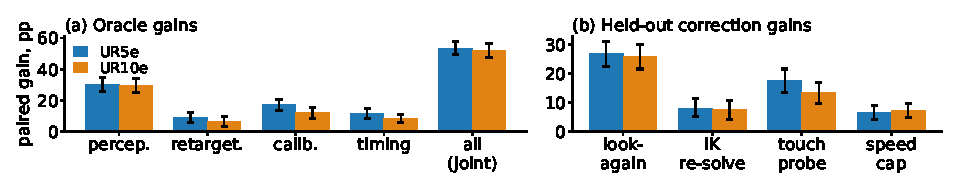
\includegraphics[width=0.95\linewidth]{figures/gap_budget_v3.pdf}
 \vspace{-1.6em}
 \caption{\textbf{Nominal error model: 500 fresh seeds per arm.} (a)~Oracle gains: perception dominates. (b)~Correction gains; look-again selected on development seeds. Bars: paired bootstrap 95\% intervals. Demonstration-derived timing changes the dominant budget (Sec.~\ref{sec:sensitivity}).}
 \label{fig:budget}
 \vspace{-0.8em}
\end{figure}

\section{Method: the Transfer Gap Budget}
\label{sec:method}

\textbf{Paired interventions.} Let $\mathcal{K}$ contain perception, retargeting, tool-frame calibration,
and execution timing. In the controlled-error study, \emph{full} includes all four perturbations;
\emph{oracle}$_k$ removes only perturbation $k$, and \emph{oracle-all} removes all four. Their ideal outputs are exact object pose, unperturbed IK, zero tool offset, and nominal timing. Each random stream is keyed by seed and component, preserving initial scenes and
unreplaced error draws across conditions. For binary success $s_c(i)$ on seed $i$ in condition $c$,
\begin{equation}
 B_k=\frac{1}{n}\sum_{i=1}^{n}\bigl(s_{\mathrm{oracle}_k}(i)-s_{\mathrm{full}}(i)\bigr),
 \qquad \Delta_{\mathrm{int}}=\sum_{k\in\mathcal{K}} B_k-B_{\mathrm{all}}.
\end{equation}
Here $B_{\mathrm{all}}$ uses the joint oracle in the same paired difference. Budgets are signed net gains:
an oracle can both rescue and lose trials. The residual shows whether summed single-stage gains exceed ($>0$) or fall below ($<0$) the joint gain; it does not allocate failures to interactions.
Oracle interventions are diagnostic, not deployment mechanisms. Budgets are conditional on the modelled error distribution, motivating measurements from demonstrations and the deployment pipeline.

\textbf{Correction selection.} The menu pairs perception with look-again, retargeting with an IK re-solve,
calibration with a modelled touch probe, and timing with a speed cap. We select
$k^\star=\arg\max_k B_k$ on development seeds, breaking ties in pipeline order. Look-again and probing reduce assumed residual errors; their manoeuvres are not simulated.

\textbf{Statistics.} Paired percentile bootstraps resample seeds with all condition scores (95\%). Demo intervals are descriptive for reused seeds, conditional on the six demonstrations for fresh seeds.

\section{Experimental Setup}

\textbf{Task.} MuJoCo simulates a fixed-base UR5e or UR10e with a Robotiq 2F-85 from MuJoCo
Menagerie~\citep{menagerie}, a 4\,cm block with $\pm$3\,cm position jitter, and a tray with 14\,cm inner width.
A scripted IK controller uses simulated contact in a UR5e-tuned layout. Success requires a lift of at least 5\,cm, release within 3\,cm of the goal,
and speed below 0.02\,m/s for 0.5\,s after release.

\textbf{A: controlled errors.} The injected magnitudes are assumptions. Both arms receive the same seed-dependent draws: Gaussian $xy$ perception error
($\sigma=\cPercSigmaCm$\,cm), joint offsets ($\sigma=\cRetSigmaDeg^\circ$ per joint),
a uniformly directed tool-frame offset with magnitude $\mathcal{U}(0,\cCalMaxCm)$\,cm, and a timing
speed-up of $\mathcal{U}(\cSpeedLo,\cSpeedHi)$ relative to robot pace. The corrections reduce perception
noise to 0.4\,cm, joint-offset noise to $0.05^\circ$, or calibration noise to 2\,mm per axis, or cap
speed-up at $3\times$. Development seeds 0--59 select look-again on both arms. After freezing the
protocol, we evaluate ten conditions on 500 fresh seeds (3000--3499) per arm: \emph{full}, four single oracles, the joint oracle, and four corrections.

\textbf{D: exploratory sensitivity.} Fresh seeds test changed error magnitudes, block sizes, jitter, layouts, and measurement-matched perception and timing (Appendix~\ref{app:sensitivity}): 200 seeds per arm, or 500 for half errors, reduced perception, and demonstration-derived timing. Correction constants are unchanged.

\textbf{B: real-video motion.} Five pick-and-place cycles from two people in two freely licensed videos,
plus one from a third person's 50\,s recording, supply motion and timing. GEM-X~\citep{gemx}
estimates hand trajectories; grasp and release frames are annotated manually. Reach and retreat
are anchored to the simulated grasp and release points, and the carry path is rotated and scaled to connect them; the scene is not reconstructed. Perception and calibration errors remain injected; no object
detector is used, and retargeting is excluded from the real-video oracle analysis. Each demo--arm pair uses 60 seeds from the revision period (1000--1059) and 60 unused seeds (5000--5059). We report leg-wise path RMSE against the retargeted reference.

\textbf{C: depth perception.} A geometric estimator fits the table plane, clusters points above it, and selects a cube and tray; its position, yaw, and size drive the controller. We test 5, 6, and 7\,cm cubes on the two arms and a third manipulator
(UR10e with a Robotiq 2F-140), with 40 seeds per size: 120 episodes per condition.

\section{Results}

\subsection{Controlled errors on two arms}

Uncorrected success is \vFiveFullK/\vFiveN{} on the UR5e and
\vTenFullK/\vTenN{} on the UR10e. Removing all errors recovers \vFiveBudAll{} and \vTenBudAll\pp{}.
Under the nominal error model, perception has the largest budget: \vFiveBudPerception{} [\vFiveBudPerceptionLo,
\vFiveBudPerceptionHi]\pp{} on the UR5e and \vTenBudPerception{} [\vTenBudPerceptionLo,
\vTenBudPerceptionHi]\pp{} on the UR10e. Calibration follows (\vFiveBudCalibration{} and \vTenBudCalibration\pp{}), then timing (\vFiveBudTiming{} and \vTenBudTiming\pp{}) and retargeting
(\vFiveBudRetargeting{} and \vTenBudRetargeting\pp{}); all single-stage intervals exclude zero
(Fig.~\ref{fig:budget}a).

The interaction residual is \vFiveInter{} [\vFiveInterLo,
\vFiveInterHi]\pp{} on the UR5e and \vTenInter{} [\vTenInterLo, \vTenInterHi]\pp{} on the UR10e.


Look-again, selected on development trials, raises success from \vFiveFullK{} to
\vFiveCorrLookAgainK/\vFiveN{} (UR5e) and \vTenFullK{} to \vTenCorrLookAgainK/\vTenN{} (UR10e); the paired gains are \vFiveCorrLookAgain{}
[\vFiveCorrLookAgainLo, \vFiveCorrLookAgainHi]\pp{} and \vTenCorrLookAgain{}
[\vTenCorrLookAgainLo, \vTenCorrLookAgainHi]\pp{}, respectively, the largest observed. Probing gives \vFiveCorrTouchProbe{} and
\vTenCorrTouchProbe\pp{}; IK re-solving and the speed cap 6--8\pp{} (Fig.~\ref{fig:budget}b).

\subsection{The dominant budget depends on the error distribution}
\label{sec:sensitivity}

The six human demonstrations span 2.0--9.4$\times$ robot pace (nominal error model: 1.0--4.5$\times$). Sampling $\mathcal{U}(2.01,9.38)$ changes the diagnosis: timing leads with budgets \tmBudA{} and \tmBudB\pp{} (\tmFullA{} and \tmFullB{} of 500 uncorrected),
\tmMarA{} [\tmMarLoA, \tmMarHiA] and \tmMarB{} [\tmMarLoB, \tmMarHiB]\pp{} above the next stage. The endpoints are measured; uniformity, calibration and retargeting magnitudes remain assumed.

Nominal, doubled-error, and shifted-layout variants retain perception as the largest point estimate; varying perception error alone changes the ranking (Fig.~\ref{fig:curve}, Appendix~\ref{app:sensitivity}).

\begin{figure}[!ht]
 \centering
 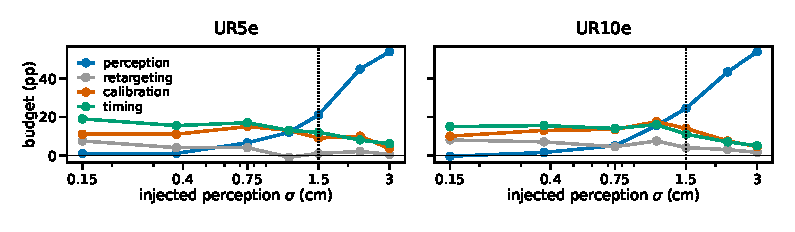
\includegraphics[width=0.9\linewidth]{figures/scale_curve.pdf}
 \vspace{-0.9em}
 \caption{Point-estimate budgets against perception error (200 seeds per point); dotted: assumed value.}
 \label{fig:curve}
 \vspace{-0.8em}
\end{figure}

Matching perception magnitudes to simulated depth measurements also changes the dominant budget between timing and perception (Appendix~\ref{app:sensitivity}).

Each 500-seed setting uses 100 development and 400 evaluation seeds.
With the demonstration-derived timing range, the budget rule picks timing: gains \tmRuleA{} and \tmRuleB\pp{}, exceeding look-again by \tmDiffA{} [\tmDiffLoA, \tmDiffHiA] and \tmDiffB{} [\tmDiffLoB, \tmDiffHiB]\pp{}.
This matches the hindsight best. Reduced perception error, alone or with doubled calibration error, also favours targeted corrections over look-again (Appendix~\ref{app:sensitivity}). Where perception dominates, the rule picks look-again and ties.

\subsection{Real-video demonstrations}

\begin{table}[!ht]
 \centering
 \caption{Successes of 60 paired seeds, uncorrected $\to$ revised stack; left seeds were reused in development, right seeds not. P1--P3: demonstrators.}
 \label{tab:demos}
 \footnotesize
 \begin{tabular}{lcccc}
  \toprule
   & \multicolumn{2}{c}{Seeds 1000--1059} & \multicolumn{2}{c}{Unused seeds} \\
  Demonstration & UR5e & UR10e & UR5e & UR10e \\
  \midrule
  P1 notebook & \dmNotebookFiveRaw $\to$ \dmNotebookFiveStack & \dmNotebookTenRaw $\to$ \dmNotebookTenStack & \frNotebookFiveRaw $\to$ \frNotebookFiveStack & \frNotebookTenRaw $\to$ \frNotebookTenStack \\
  P1 markers & \dmMarkersFiveRaw $\to$ \dmMarkersFiveStack & \dmMarkersTenRaw $\to$ \dmMarkersTenStack & \frMarkersFiveRaw $\to$ \frMarkersFiveStack & \frMarkersTenRaw $\to$ \frMarkersTenStack \\
  P1 orange marker & \dmOrangeFiveRaw $\to$ \dmOrangeFiveStack & \dmOrangeTenRaw $\to$ \dmOrangeTenStack & \frOrangeFiveRaw $\to$ \frOrangeFiveStack & \frOrangeTenRaw $\to$ \frOrangeTenStack \\
  P1 notepad & \dmNotepadFiveRaw $\to$ \dmNotepadFiveStack & \dmNotepadTenRaw $\to$ \dmNotepadTenStack & \frNotepadFiveRaw $\to$ \frNotepadFiveStack & \frNotepadTenRaw $\to$ \frNotepadTenStack \\
  P2 box (own stack) & \dmPTwoOwnFiveRaw $\to$ \dmPTwoOwnFiveStack & \dmPTwoOwnTenRaw $\to$ \dmPTwoOwnTenStack & \frPTwoOwnFiveRaw $\to$ \frPTwoOwnFiveStack & \frPTwoOwnTenRaw $\to$ \frPTwoOwnTenStack \\
  P2 box (P1 stack) & \dmPTwoPOneFiveRaw $\to$ \dmPTwoPOneFiveStack & \dmPTwoPOneTenRaw $\to$ \dmPTwoPOneTenStack & \frPTwoPOneFiveRaw $\to$ \frPTwoPOneFiveStack & \frPTwoPOneTenRaw $\to$ \frPTwoPOneTenStack \\
  P3 recording (P1 stack) & \dmOwnFiveRaw $\to$ \dmOwnFiveStack & \dmOwnTenRaw $\to$ \dmOwnTenStack & \frOwnFiveRaw $\to$ \frOwnFiveStack & \frOwnTenRaw $\to$ \frOwnTenStack \\
  \bottomrule
 \end{tabular}
 \vspace{-0.8em}
\end{table}

These experiments transfer human motion and timing into simulation. The notebook demo fails uncorrected on both arms at about $6\times$ robot pace. Sequential diagnosis
selects a $3\times$ speed cap, look-again, calibration probing, then a tighter $2\times$ cap; with the revised retreat the stack reaches
\dmNotebookFiveStack/60 and \dmNotebookTenStack/60 (Table~\ref{tab:demos}), and RMSE to the retargeted
reference falls from \dmPathRawFive{} to \dmPathFixFive\,cm (UR5e) and \dmPathRawTen{} to \dmPathFixTen\,cm (UR10e).

The original stack scored \dmVOneMax/60 on all \dmVOneDemos{} additional P1 cycles because the copied retreat paths intersected the tray. On P2, the same retreat caused UR5e success to drop from \dmVFourRaw/60 to \dmVFourStack/60.
We therefore added a 5\,cm lift before retreating along the human path (selected on development seeds 0--19; path-RMSE cost \dmCostMin--\dmCostMax\,cm).
The revised P1 stack transfers to P2 and P3 without retuning; P1 markers remain difficult on the UR10e (\dmMarkersTenStack/60).
Seeds 1000--1059 informed revision; those columns are exploratory. On unused seeds 5000--5059, every cell improves: the revised stack reaches \frStackMin--60/60 against at most \frRawMax/60 uncorrected,
all paired intervals exclude zero, and P1 markers on the UR10e reach \frMarkersTenStack/60.

\subsection{Depth perception}

All \pcBarMet/\pcBarCells{} pre-declared acceptance cells reach the 90\% point-estimate threshold across three manipulators. Separate notebook-path comparisons show close depth and ground-truth results. Calibration stress and occlusion expose limits (Appendix~\ref{app:depth}); physical-camera transfer remains untested.

\section{Limitations and Conclusion}
\label{sec:limits}

The budget is conditional on the assumed or measured error distribution. Timing ranges come from six demonstrations and depth-error magnitudes from simulation; calibration and retargeting errors and correction models remain assumed. The study uses one simulated task, scripted controllers, and a UR5e-tuned layout; layout shifts leave the table and task fixed. Three demonstrators and unreconstructed scenes limit generalisation. Look-again and probing manoeuvres and their time costs are not simulated. Real-robot performance is untested.

The Transfer Gap Budget diagnoses recoverable transfer failures through paired interventions. Perception dominates under the nominal error model; demonstration-derived timing makes timing dominant. Corrections and a revised retreat improve human-video transfer on unused seeds. These results suggest that the value of additional human data should be evaluated together with the transfer-error distribution it induces, since changes in timing, motion, or scene variation can shift the dominant transfer bottleneck.

\textbf{Author responsibility.} Reported values were checked against available experimental records; the authors are responsible for the work.

\clearpage
\acknowledgments{Omitted for blind review.}
\bibliography{refs}

\clearpage
\appendix
\section{Additional simulation results}

\subsection{Additional error-distribution sensitivity}
\label{app:sensitivity}
\textbf{E: exploratory sensitivity.} Fresh seeds (200 per arm unless stated) test A's oracles and selected corrections with errors scaled 0.5$\times$ (500 seeds) or 2$\times$, 3 or 5\,cm blocks, $\pm$5\,cm jitter, tray or block shifts of 8--10\,cm,
perception error scaled 0.1--2$\times$, cut to 25\% alone or with doubled calibration error (500 seeds), matched to simulated depth-error measurements, and timing spanning demonstration speeds (500 seeds). Correction constants are unchanged.

Perception has the largest point-estimate budget at nominal and doubled errors, with 3 or 5\,cm blocks, $\pm$5\,cm jitter (ten cells), and moved tray or block (six cells).
At $0.5\times$ errors (\ehFullFive{} and \ehFullTen{} of 500 uncorrected) it still leads, by \ehMarginFive\pp{} [\ehMarginLoFive, \ehMarginHiFive] over calibration on both arms.
Varying only perception error (Fig.~\ref{fig:curve}), perception leads from the assumed 1.5\,cm upward; at 0.75$\times$ and below calibration and timing take over.

Tying magnitudes to measurements changes the ranking. The simulated depth estimator's block-position error is \mmNom\,mm RMS per axis with exact camera calibration, and \mmHalf{} and \mmOne\,mm with $0.5^\circ$/5\,mm and $1^\circ$/10\,mm calibration error.
Injected as the perception error, these give perception budgets of \DnNomPercFive{} and \DnNomPercTen\pp{}, \DnHalfPercFive{} and \DnHalfPercTen\pp{} (timing leads at both), and \DnOnePercFive{} and \DnOnePercTen\pp{} (perception leads).

Each 500-seed correction setting uses 100 development and 400 evaluation seeds.
With perception error cut to 25\%, the rule picks timing: gains \rpA{} and \rpB\pp{} versus \rlA{} and \rlB\pp{} for look-again, a difference of \rdA{} [\rdAlo, \rdAhi] and \rdB{} [\rdBlo, \rdBhi]\pp{}.
It trails hindsight-best calibration by 1.2 and 1.5\pp{} (difference intervals include zero).
With calibration error also doubled, it picks calibration: gains \rcA{} and \rcB\pp{} versus about zero for look-again, differences \reA{} [\reAlo, \reAhi] and \reB{} [\reBlo, \reBhi]\pp{}.
The doubled-calibration setting matches the hindsight best.


\subsection{Depth comparison details}
\label{app:depth}
All \pcBarMet/\pcBarCells{} pre-declared acceptance cells reach the 90\% point-estimate threshold (\pcBarMin--\pcN{} of \pcN{} episodes), covering yaw, distractors, depth noise, occlusion with a retry, and combined stressors on three manipulators.
Report-only stress tests expose limits: $2^\circ$/20\,mm calibration error gives \pcCalibTwoFive/\pcN{} on the UR5e, and occlusion without retry \pcArmMin--\pcArmMax/\pcN{}.
For the notebook path at robot pace, depth versus ground-truth success is \spKFiveDepth{} versus \spKFiveTruth/\spN{} (UR5e), \spKTenDepth{} versus \spKTenTruth/\spN{} (UR10e), and \spKKaiDepth{} versus \spKKaiTruth/\spN{} (UR10e with a Robotiq 2F-140). Depth success is 0.8--1.7\pp{} higher, with path RMSE within 0.01\,cm. All three arms meet the point-estimate margins of 10\pp{} success loss and 0.5\,cm added RMSE (no inferential non-inferiority test). These simulated measurements inform the sensitivity analysis; physical-camera transfer remains untested.

\subsection{Exploratory humanoid runtime sensitivity}
\label{app:g1}
A Unitree G1 with Dex3 hands uses SONIC whole-body control~\citep{sonic2025}. We score grasp (5\,cm lift with contact) and placement within 5\,cm of the goal; we do not estimate stage budgets here.
With IK-planned targets, the same frozen closed-loop controller places \giHostPlace/\giN{} objects in a volume-based installation and \giImgPlace/\giN{} in a packaged container (same GPU, seeds 1200--1239; discordant placements \giOnlyImg{} to \giOnlyHost{}, exact McNemar $p=\giP$). Code and environment checks did not identify the cause; a four-seed MuJoCo 3.15.0 rebuild (\mjGraspNew/\mjNNew{} lifts versus \mjGraspOld/\mjNOld{} on 3.14.0) also changed \texttt{filelock}. This unresolved runtime sensitivity is exploratory and does not support a causal explanation or the main Transfer Gap Budget claims.
\end{document}
